% A simple Pentagon with TiKZ
% Author: Christoph Gerum <gerum@informatik.uni-tuebingen.de>

\documentclass{article}

\usepackage{tikz}
\usepackage{subfig}

\begin{document}

  \begin{figure}[htbp]
    \begin{center}
      \subfloat[Ohne Pipelineing]{
        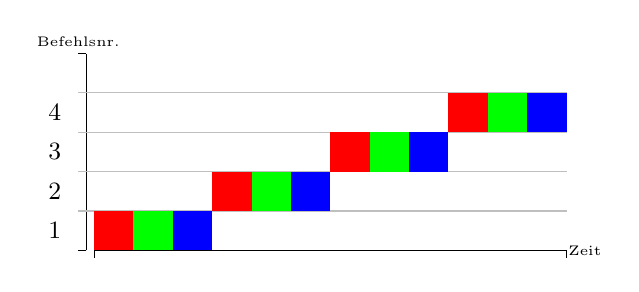
\begin{tikzpicture}
          %Achsen
          \draw (0cm,0cm) -- (6cm,0cm);  %Abzisse
          \draw (0cm,0cm) -- (0cm,-0.1cm);
          \draw (6cm,0cm) -- (6cm,-0.1cm) node at (5.9cm, 0cm) [right] {\tiny{Zeit}};
          
          \draw (-0.1cm,0cm) -- (-0.1cm,2.5cm);  %Ordinate
          \draw (-0.1cm,0cm) -- (-0.2cm,0cm); 
          \draw (-0.1cm,2.5cm) -- (-0.2cm,2.5cm) node at (-0.2,2.65) {\tiny{Befehlsnr.}};
          
          \foreach \x in {1,...,4}
          \draw[gray!50, text=black] (-0.2 cm,\x*0.5 cm) -- (6 cm,\x*0.5 cm) node at (-0.5 cm,\x*0.5 cm - 0.25cm) {\small{\x}};
          
          \foreach \pos in {0,0.5,1,1.5}{
            \foreach \dx/\color in {0/red,0.5/green,1/blue}{
              \fill [fill=\color] (\pos * 3 cm+\dx cm,\pos cm) rectangle (\pos * 3 cm + \dx cm + 0.5 cm, \pos cm + 0.5 cm);
            }
          }
          
        \end{tikzpicture}
      }
      \subfloat[Mit Pipelineing]{
        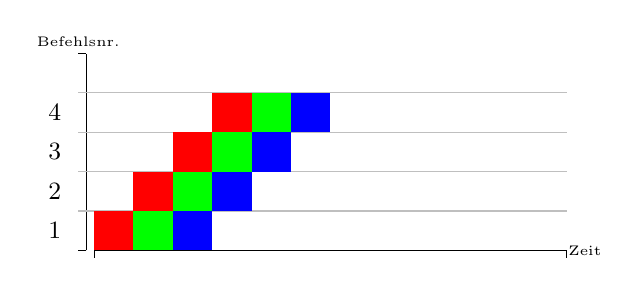
\begin{tikzpicture}
          %Achsen
          \draw (0cm,0cm) -- (6cm,0cm);  %Abzisse
          \draw (0cm,0cm) -- (0cm,-0.1cm);
          \draw (6cm,0cm) -- (6cm,-0.1cm) node at (5.9cm, 0cm) [right] {\tiny{Zeit}};
          
          \draw (-0.1cm,0cm) -- (-0.1cm,2.5cm);  %Ordinate
          \draw (-0.1cm,0cm) -- (-0.2cm,0cm); 
          \draw (-0.1cm,2.5cm) -- (-0.2cm,2.5cm) node at (-0.2,2.65) {\tiny{Befehlsnr.}};
          
          \foreach \x in {1,...,4}
          \draw[gray!50, text=black] (-0.2 cm,\x*0.5 cm) -- (6 cm,\x*0.5 cm) node at (-0.5 cm,\x*0.5 cm - 0.25cm) {\small{\x}};
          
          \foreach \pos in {0,0.5,1,1.5}{
            \foreach \dx/\color in {0/red,0.5/green,1/blue}{
              \fill [fill=\color] (\pos cm+\dx cm,\pos cm) rectangle (\pos cm + \dx cm + 0.5 cm, \pos cm + 0.5 cm);
            }
          }
          
        \end{tikzpicture}
      }
    \end{center}
    
    \caption{Auswirkung von Pipelining auf die Ausführungszeit}
    \label{fig:pipelining}
  \end{figure}

\end{document}
